\documentclass[8pt,a4paper,compress]{beamer}

\usepackage{/home/siyer/lib/slides}

\title{Course Mechanics}
\date{}

\begin{document}
\begin{frame}
\vfill
\titlepage
\end{frame}

\section{Website}
\begin{frame}[fragile]
\pause

http://www.swamiiyer.net/cs451
\end{frame}

\section{Goal}
\begin{frame}[fragile]
\pause

Theory
\begin{itemize}
\pause
\item Scan a program into a stream of tokens

\pause
\item Parse a program making its syntactic structure explicit

\pause
\item Analyze and generate code for various programming constructs

\pause
\item Allocate physical registers to a program expressed in terms of virtual registers
\end{itemize}

\pause\bigskip

Practice
\begin{itemize}
\pause
\item Develop a compiler (called \jmm) in Java for a significantly large subset (also called \jmm) of the Java programming language 
\end{itemize}


\end{frame}

\section{Prerequisites}
\begin{frame}[fragile]
\pause

CS310 and CS420 or CS622
\end{frame}

\section{Instructor}
\begin{frame}[fragile]
\pause

Swami Iyer (\href{siyer@cs.umb.edu}{siyer@cs.umb.edu})

\pause\bigskip

Office Hours: Tue Thu 10:00 AM -- Noon (S-03-0079)
\end{frame}

\section{Class}
\begin{frame}[fragile]
\pause

\visible<2->{
\tcbox[enhanced,drop shadow southwest,sharp corners,size=fbox,colback=white]{
\begin{tabular}{ll}
\textbf{When} & \textbf{Where} \\ \hline \\
Tue Thu 4:00 PM -- 5:15 PM & W--01--0004 \\ 
\end{tabular}
}
}
\end{frame}

\section{Text}
\begin{frame}[fragile]
\pause

\begin{center}
\visible<2->{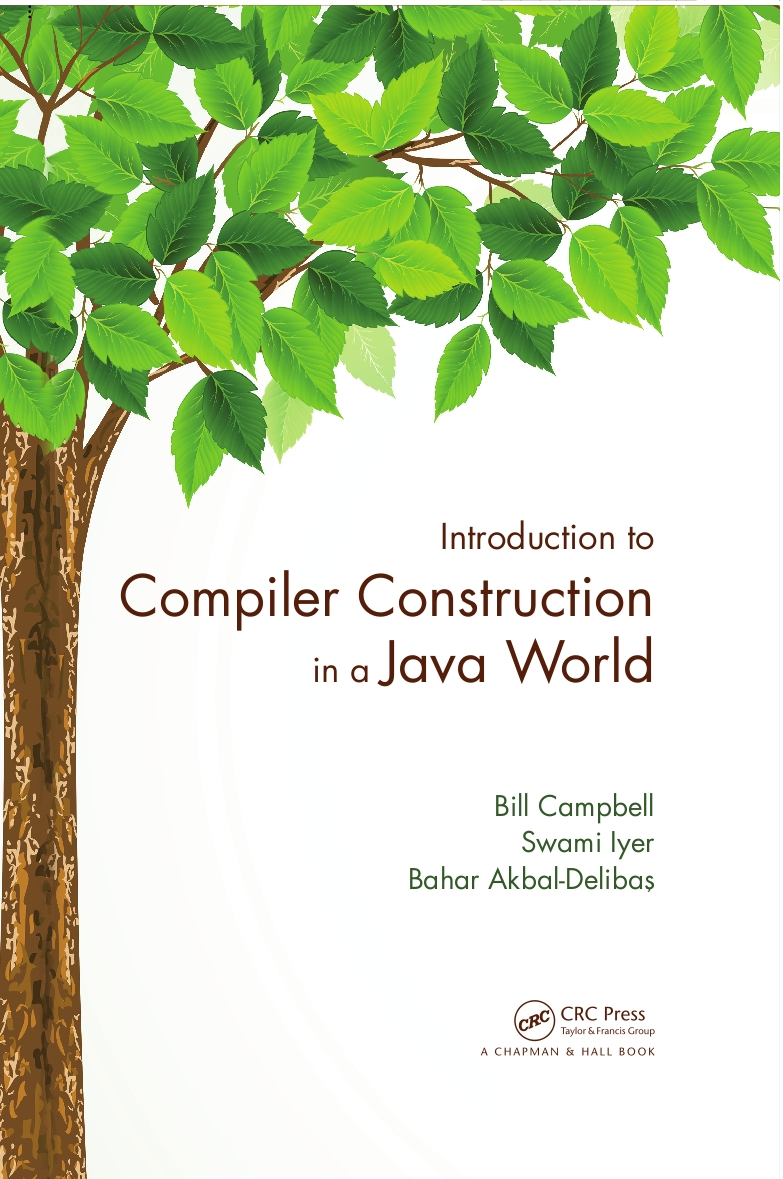
\includegraphics[scale=0.26]{figures/text.png}}
\end{center}
\end{frame}

\section{Grading}
\begin{frame}[fragile]
\pause

\visible<2->{
\tcbox[enhanced,drop shadow southwest,sharp corners,size=fbox,colback=white]{
\begin{tabular}{ll}
\textbf{Item} & \textbf{\% of Final Grade} \\ \hline \\
Projects (1, 2, 3, and 5 and best of 4 and 6) & 45 \\
Exams (best 2 of 3) & 50 \\
Attendance & 5 \\
\end{tabular}
}
}

\pause\bigskip

\visible<3->{
\tcbox[enhanced,drop shadow southwest,sharp corners,size=fbox,colback=white]{
\begin{tabular}{ll}
\textbf{\% Score} & \textbf{Grade} \\ \hline \\
$[93, 100]$ & A \\
$[90, 93)$ & A- \\
$[87, 90)$ & B+ \\
$[83, 87)$ & B \\
$[80, 83)$ & B- \\
$[77, 80)$ & C+ \\
$[73, 77)$ & C \\
$[70, 73)$ & C- \\
$[67, 70)$ & D+ \\
$[63, 67)$ & D \\
$[60, 63)$ & D- \\
$[0, 60)$ & F \\
\end{tabular}
}
}
\end{frame}

\section{Software}
\begin{frame}[fragile]
\pause

Estalee (attendance platform)

\pause\bigskip

Piazza (Q\&A platform)

\pause\bigskip

Gradescope (grading platform)

\pause\bigskip

Programming environment (linux-based virtual machine)
\end{frame}

\section{Policies}
\begin{frame}[fragile]
\pause

Classroom

\pause\bigskip

Piazza

\pause\bigskip

Collaboration

\pause\bigskip

Student code of conduct

\pause\bigskip

Accommodations for students with disabilities
\end{frame}

\section{Course Website}
\begin{frame}[fragile]
\pause

Announcements (landing page)

\pause\bigskip

Course Info

\pause\bigskip

Calendar

\pause\bigskip

Lecture Material 

\pause\bigskip

Projects

\pause\bigskip

Resources
\end{frame}

\section{Immediate Action Items}
\begin{frame}[fragile]
\pause

Sign up for Estalee

\pause\bigskip

Sign up for Piazza

\pause\bigskip

Sign up for Gradescope

\pause\bigskip

Sign up for CS account

\pause\bigskip

Setup the programming environment
\end{frame}

\end{document}
